% ============================================================
% Assignment 5 — Ines Casado Vela
% Hard majority voting
% Images are expected in the root Overleaf folder `pics/`.
% ============================================================

\subsection{Hard Majority Voting}

For the hard-voting ensemble, we combined the predictions of the three transformer models
used in Assignment~4: BERT, HateBERT and fBERT. Logistic Regression was not included because
its performance, especially in the cross-domain setting, was clearly lower than that of the
three transformer models.

The method is simple: each model predicts either the non-offensive or offensive class, and the
final prediction is the label selected by at least two of the three models. Since we use three
models, there are no ties. We applied the same procedure separately to the in-domain and
cross-domain predictions from Assignment~4. No additional training was needed for this
ensemble.

We evaluated the ensemble on the same 860 OLID test examples used in Assignment~4. We report
accuracy, macro-averaged precision, recall and F1, together with the per-class scores and the
confusion matrices.

\subsubsection{Results}

Table~\ref{tab:hard-voting-results} shows the results of hard majority voting. In the
in-domain setting, the ensemble reaches a macro-F1 score of 0.8018. In the cross-domain
setting, the score decreases to 0.7863. This is an absolute decrease of 0.0155 macro-F1
points, or approximately 1.93\% relative to the in-domain result.

\begin{table}[ht]
\centering
\caption{Hard majority voting results on the OLID test set.}
\label{tab:hard-voting-results}
\begin{tabular}{lrrrrrrrr}
\hline
Setting & Acc. & Macro-P & Macro-R & Macro-F1 & F1 (0) & P (1) & R (1) & F1 (1) \\
\hline
In-domain    & 0.8407 & 0.8022 & 0.8014 & 0.8018 & 0.8896 & 0.7155 & 0.7125 & 0.7140 \\
Cross-domain & 0.8349 & 0.8005 & 0.7757 & 0.7863 & 0.8882 & 0.7333 & 0.6417 & 0.6844 \\
\hline
\end{tabular}
\end{table}

The confusion matrices show a similar pattern. In-domain, the ensemble produces 552 true
negatives, 68 false positives, 69 false negatives and 171 true positives. In the cross-domain
setting, there are 564 true negatives, 56 false positives, 86 false negatives and 154 true
positives. The main change is therefore in the offensive class: its recall decreases from
0.7125 to 0.6417, meaning that more offensive examples are missed in the cross-domain setup.

\begin{figure}[ht]
\centering
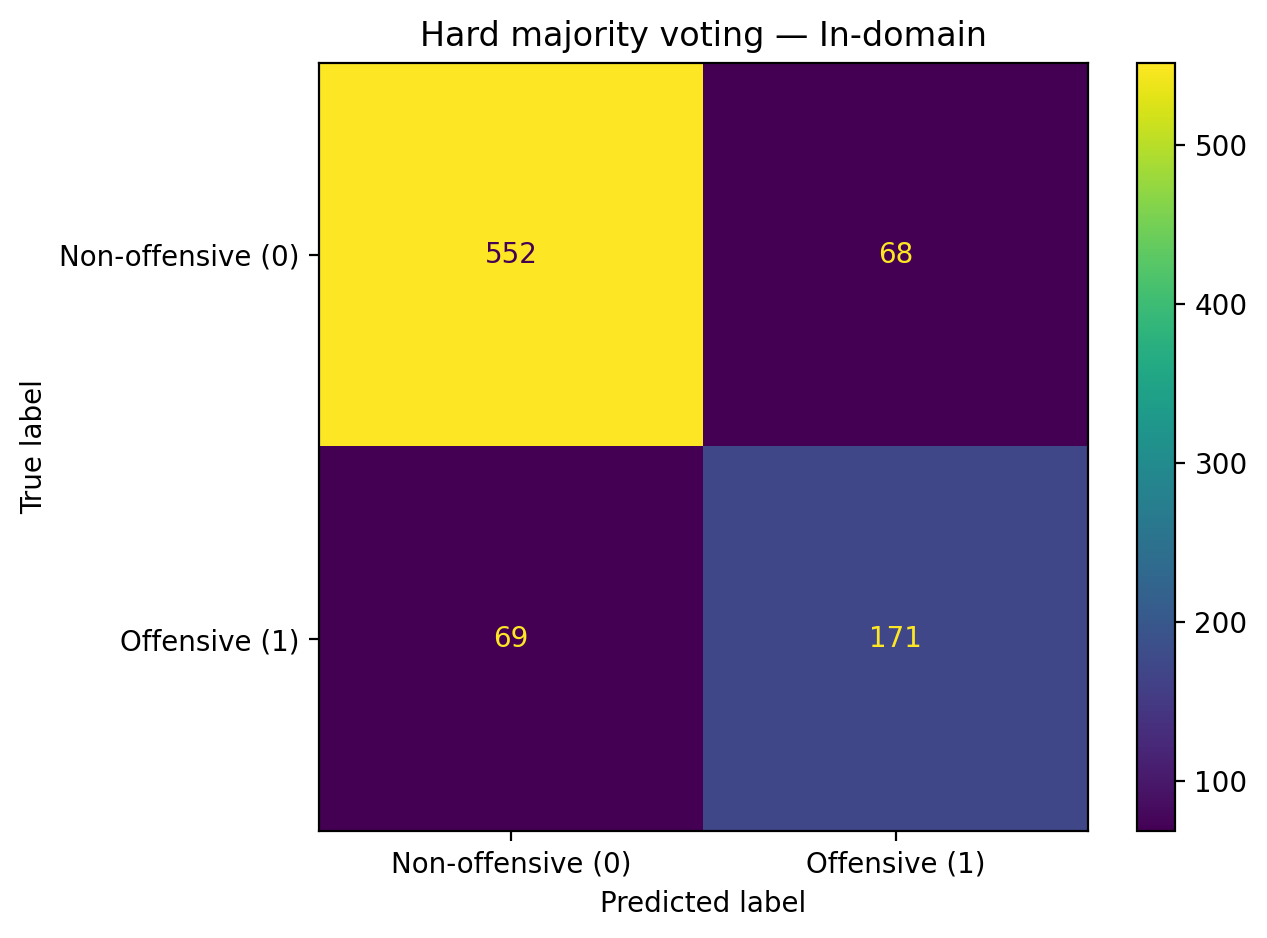
\includegraphics[width=0.47\textwidth]{pics/hard_voting_confusion_in_domain.png}
\hfill
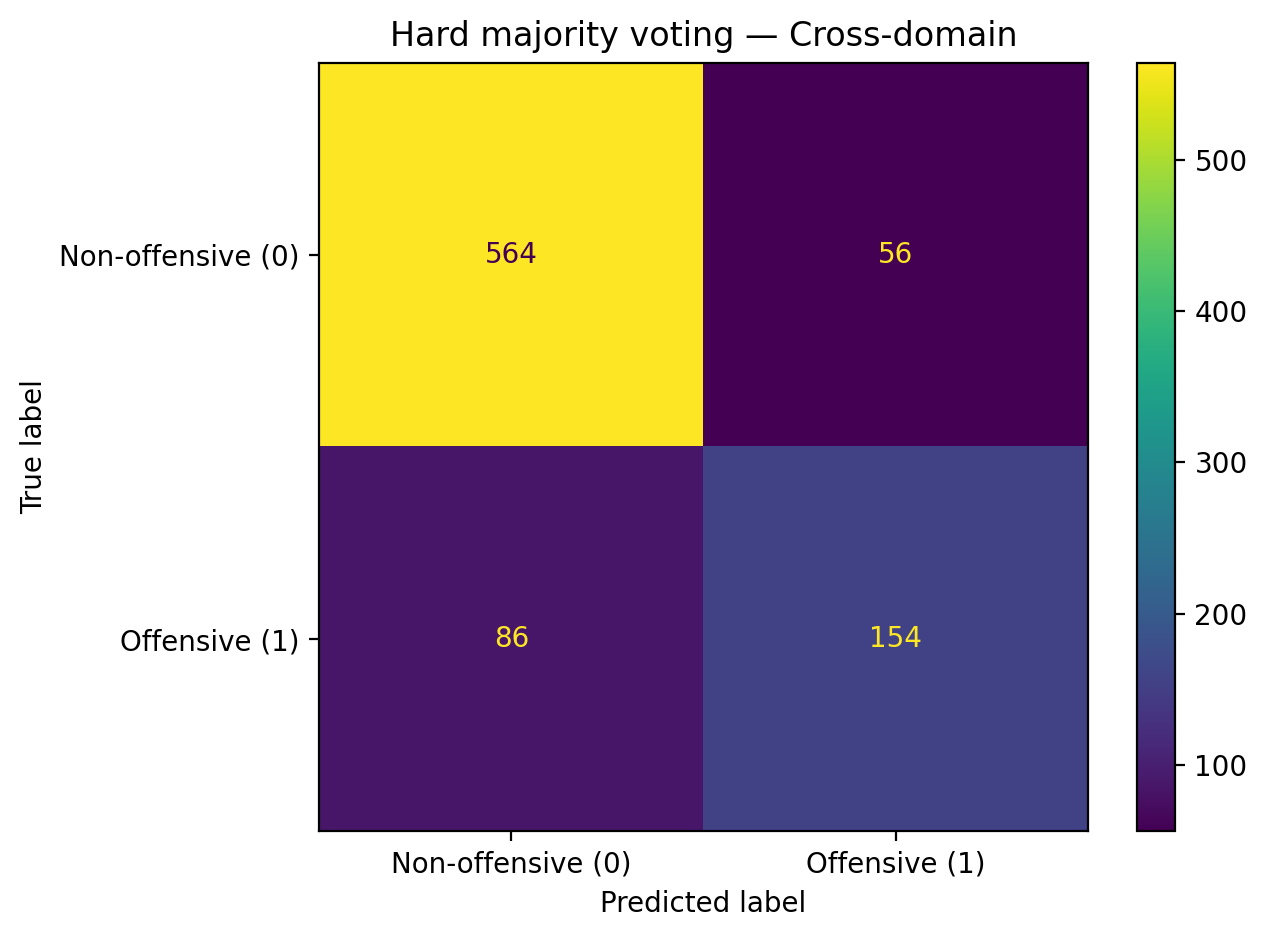
\includegraphics[width=0.47\textwidth]{pics/hard_voting_confusion_cross_domain.png}
\caption{Confusion matrices for hard majority voting in the in-domain (left) and
cross-domain (right) settings.}
\label{fig:hard-voting-cm}
\end{figure}

Hard voting does not improve on the strongest individual model from Assignment~4. fBERT
obtained macro-F1 scores of 0.8033 in-domain and 0.8088 cross-domain, while hard voting
obtains 0.8018 and 0.7863. The difference is very small in-domain, but it is larger in the
cross-domain setting.

A possible explanation is that the three transformer models often make the same prediction.
They agree on 707 of the 860 test examples in-domain and on 647 examples cross-domain.
Therefore, in many cases the ensemble simply reproduces the same decision as the individual
models instead of correcting an error. This also means that the benefit of majority voting is
limited when the models behave similarly.

The cross-domain result is also affected by the fact that fBERT was clearly stronger than
BERT and HateBERT in Assignment~4. Since hard voting gives all three models the same weight,
there are cases where a correct fBERT prediction can be overruled by the other two models.
Even so, the ensemble remains competitive and performs better cross-domain than BERT and
HateBERT individually.